\documentclass[thesis,fonts=libertine]{cluu}

\usepackage[style=cluu]{biblatex}
\usepackage{amsmath}

\DeclareMathOperator*{\argmax}{arg\,max}
\DeclareMathOperator*{\argmin}{arg\,min}

\usepackage{tikz}
\usepackage{graphicx}
\usepackage{url}
\usepackage{listings}
\usepackage{siunitx}
\usepackage[boxed, noline]{algorithm2e}
\usepackage{pgfplots}
\usepackage{pdfpages}

\graphicspath{ {figures/} }
\addbibresource{thesis.bib}

\usepackage{pythonhighlight}    % for \inputpython at the end

\begin{document}
\author{Shifei Chen}
\supervisors{Ali Basirat, Uppsala University}
\title{Cross-lingual Word Embeddings Beyond Zero-shot Machine Translation}

\maketitle

\begin{abstract}
  This thesis explored the possibility of transferring learning from training languages to completely unknown languages in a multilingual neural machine translation system. Using cross-lingual word embeddings as the only knowledge source, we observed little transferability between highly-related languages from our experiment. We also discussed the shortcomings of multilingual neural machine translation architecture that could contribute to the low transferability and provided suggestions that could better share embedding layers from the training language to unknown languages.
\end{abstract}

\tableofcontents

\addchap{Preface}

This thesis was finished under the supervision of Ali Basirat. I would like 
to thank him first for his guidance, inspiration and passion.

The Saga supercomputer owned by UNINETT Sigma2 hosted all of the experiment in this thesis.\footnote{\url{https://www.sigma2.no/systems\#saga}} Without it this thesis would not be possible.

Thank you Mr. Anders Wall and everyone in the Anders Wall Scholarship Foundation for sponsoring my Master's study. This opportunity led me to meet everyone in the Master Programme in Language Technology, from whom I have learned a lot during the 2-years journey.

Last but not least, I would like to say a thank you to my parents for their unconditional love and support; to all of my friends for the unique memories we have created; and to my girlfriend, who has always been next to me when the virus made everything unusual.

% by using \addchap instead of \chapter this preface isn't numbered.

\chapter{Introduction}

Multilingual neural machine translation (NMT) aims to train a single translation model for multiple languages \parencite{Johnson:2016aa,aharoni-etal-2019-massively}. One of its appealing points is zero-shot translation, which enables translations between unseen language pairs when knowledge from one language is transferred to another language by the model's shared parameters. Even though both source and target languages in such an unseen pair should still be in the set of training languages, a multilingual NMT system with zero-shot learning is still attractive as it lowers the cost of obtaining expensive parallel data, particularly when translating low-resource languages.

The success of zero-shot translation depends on the model's ability to learn language invariant features \parencite{Arivazhagan:2019aa}. \textcite{Kim:2019aa} believes the embedding layers is one of the critical components responsible for learning such generalized features in a multilingual NMT system. By contrast, \textcite{aji-etal-2020-neural} concluded that sharing the embedding layer alone is not enough for transfer learning in zero-shot machine translation. No matter embedding layers are essential to zero-shot learning or not, they both showed that it would positively impact the multilingual model's transferability as long as the embeddings layers are aligned between the source language and the target language.

By far, research on zero-shot learning in multilingual NMT has been mostly restricted to the limited scope of unseen language pairs. There is less discussion about the multilingual NMT transferability on completely unknown languages that have never been in the training data. This thesis studies the importance of word representation in the multilingual NMT transfer model based on the pre-trained cross-lingual word embeddings \parencite{Bojanowski:2016aa,Ammar:2016aa,Joulin:2018aa,Ruder:2019aa} and pushes it further than unseen language pairs --- examining the transferability of a multilingual NMT when it is applied to a new test language. Despite the debate on whether cross-lingual word embeddings are vital when transferring information in zero-shot translation, it is generally acknowledged that cross-lingual word embeddings are beneficial for the model's transferability. Thus we will use cross-lingual word embeddings as the source of transfer knowledge to the test languages and leave the translation model's shared parameters to model the interrelationships between the training languages.

We hypothesize that a multilingual NMT model trained with pre-trained cross-lingual word embeddings should transfer reasonably even to a completely unknown language. Although from the experiment results, cross-lingual word embeddings transfer only marginally between closely related languages. Our findings are in line with \textcite{aji-etal-2020-neural} and indicate that some regularization is necessary to transfer the embedding layers between languages. Furthermore, when using aligned pre-trained word embeddings as the only transferable knowledge source, the performance will be negatively affected by the transformed output vector space, which needs to be countered in the future.

The rest of the thesis is organized as below:

Chapter \ref{chap:background} talks about the background and previous works when working in the transferability of cross-lingual word embeddings scope, including information about cross-lingual word embeddings and multilingual neural machine translation. After that, Chapter \ref{chap:research_question} describe the research question. Chapter \ref{chap:method} introduces our experiment method, whose result are discussed and analyzed in Chapter \ref{chap:results}. Finally, Chapter \ref{chap:conclusion} gives out our conclusion. We also show samples of our multilingual NMT model in Appendix \ref{chap:example_output}.

\chapter{Background}
\label{chap:background}

\section{Word Embeddings}
\subsection{Representing Words by Vectors}

In Natural Language Processing, people need to represent words in the forms that are more efficient for computers to process. The idea started with statistical language modeling, which was introduced to Machine Translation in the early nighties \parencite{brown-etal-1990-statistical}, followed by \textcite{bengio2003neural} who powered statistical langauge modeling with neural networks. \textcite{Mikolov:2013aa} introduced Word2Vec, which encapsulates words and their latent information into vectors. Besides the benefit that it simplifies representation and storage of words for computers, it enables the possibilities to calculate words and their semantic meanings just as vectors.

Take an example of vocabulary $V=\{\text{water}, \text{hydrogen},  \text{oxygen}$\}, if we convert these words into vectors, we could have an equation of

\begin{equation}
  \label{equa:semantic_vectors}
  \vec{w}=\vec{h}+\vec{o}
\end{equation}

\noindent where $\vec{w} = \text{vec}(\text{water})$, $\vec{h} = \text{vec}(\text{hydrogen})$ and $\vec{o} = \text{vec}(\text{oxygen})$. From either the individual word (vector) prespective and the united equation prespective, Equation \ref{equa:semantic_vectors} is meaningful mathematically and semantically.

Mathematically, we can observe a small geometric angle between $\vec{h}$ and $\vec{o}$. From the cosine similarity definition below,

\begin{equation*}
  \text{sim}(x, y) = \cos(\theta) = \frac{x \cdot y}{||x||||y||}
\end{equation*}

\begin{figure}
  \centering
  \tikzset{every picture/.style={line width=0.75pt}} %set default line width to 0.75pt
  \begin{tikzpicture}[x=0.75pt,y=0.75pt,yscale=-1,xscale=1]
    %uncomment if require: \path (0,256); %set diagram left start at 0, and has height of 256

    %Shape: Axis 2D [id:dp40983147480798976]
    \draw  (49,221.35) -- (260.5,221.35)(70.15,31) -- (70.15,242.5) (253.5,216.35) -- (260.5,221.35) -- (253.5,226.35) (65.15,38) -- (70.15,31) -- (75.15,38)  ;
    %Straight Lines [id:da3468248594605029]
    \draw [color={rgb, 255:red, 74; green, 144; blue, 226 }  ,draw opacity=1 ]   (70.15,221.35) -- (91.04,133.95) ;
    \draw [shift={(91.5,132)}, rotate = 463.44] [color={rgb, 255:red, 74; green, 144; blue, 226 }  ,draw opacity=1 ][line width=0.75]    (10.93,-3.29) .. controls (6.95,-1.4) and (3.31,-0.3) .. (0,0) .. controls (3.31,0.3) and (6.95,1.4) .. (10.93,3.29)   ;
    %Straight Lines [id:da268618270283273]
    \draw [color={rgb, 255:red, 208; green, 2; blue, 27 }  ,draw opacity=1 ]   (70.15,221.35) -- (127.85,182.12) ;
    \draw [shift={(129.5,181)}, rotate = 505.79] [color={rgb, 255:red, 208; green, 2; blue, 27 }  ,draw opacity=1 ][line width=0.75]    (10.93,-3.29) .. controls (6.95,-1.4) and (3.31,-0.3) .. (0,0) .. controls (3.31,0.3) and (6.95,1.4) .. (10.93,3.29)   ;
    %Straight Lines [id:da46956564149919644]
    \draw [color={rgb, 255:red, 245; green, 166; blue, 35 }  ,draw opacity=1 ]   (70.15,221.35) -- (131.69,192.84) ;
    \draw [shift={(133.5,192)}, rotate = 515.14] [color={rgb, 255:red, 245; green, 166; blue, 35 }  ,draw opacity=1 ][line width=0.75]    (10.93,-3.29) .. controls (6.95,-1.4) and (3.31,-0.3) .. (0,0) .. controls (3.31,0.3) and (6.95,1.4) .. (10.93,3.29)   ;

    % Text Node
    \draw (83,108) node [anchor=north west][inner sep=0.75pt]   [align=left] {$\vec{w}$};
    % Text Node
    \draw (132,166) node [anchor=north west][inner sep=0.75pt]   [align=left] {$\vec{h}$};
    % Text Node
    \draw (138,183) node [anchor=north west][inner sep=0.75pt]   [align=left] {$\vec{o}$};
  \end{tikzpicture}
  \caption{Illustraion of a vector space where Equation \ref{equa:semantic_vectors} exists.}
  \label{fig:semantic_vectors}
\end{figure}

\noindent the smaller the angle $\theta$ between $\vec{h}$ and $\vec{o}$ is, the higher their cosine similarity is. In other words, when $\theta$ is zero, the cosine similarity $\text{sim}(x, y) \in [0, 1]$ will also approach its upper bound one. Also, as illustrated in Figure \ref{fig:semantic_vectors}, vector $\vec{w}$ is roughly the sum of vector $\vec{h}$ and $\vec{o}$.

Semantically, words ``hydrogen'' and ``oxygen'' are similar since they point to two chemical elements. Adding them together is like how people would ignite the mixture of hydrogen and oxygen to produce water.

To turn words into vectors, one could use a simple one-hot encoding. Like in the example above we could make $\vec{w}=[1, 0, 0]$. However, these one-hot vectors cannot capture any latent semantic information between different words, nor to reflect the inflections between stems and their variants. Such as the  word ``hydrogen'' and its stem ``hydro-''.

Recent vectorized word representations (word embeddings) were learned by neural networks.  Compared to the naive one-hot vectors, word embeddings contains affluent information that links word together. One of the examples is Word2Vec, which learns word representations through a Skip-gram model or a Continuous Bag of Words (CBOW) model \parencite{Mikolov:2013ab}. Both models are shown in Figure \ref{fig:skip_gram_and_cbow}.

\begin{figure}
  \centering
  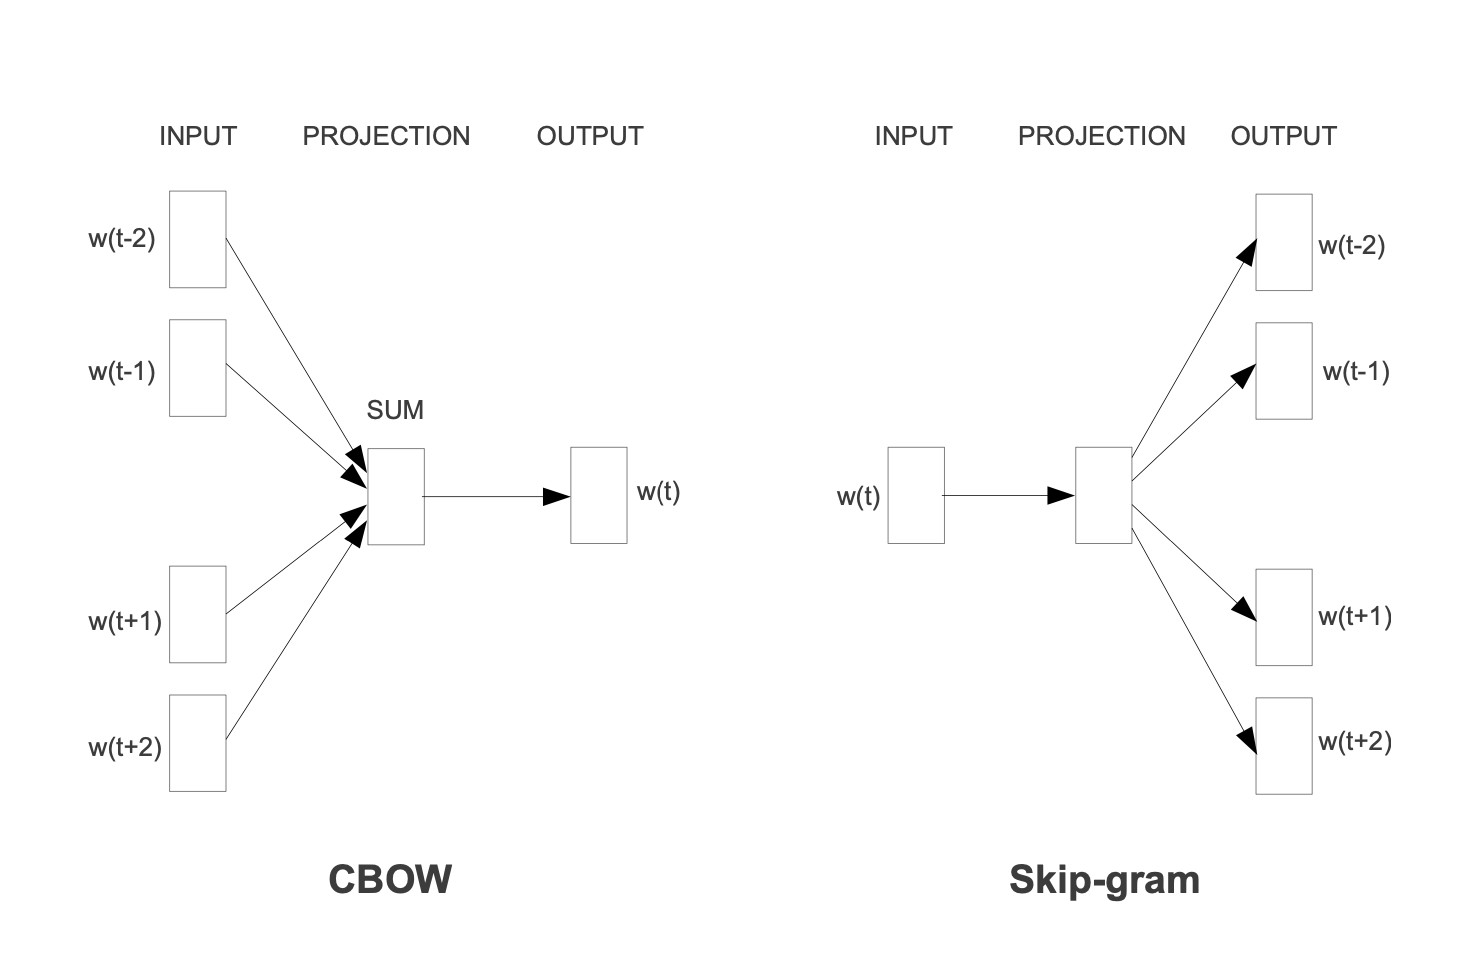
\includegraphics[width=0.8\textwidth]{skip_gram_and_cbow_models.png}
  \caption{The Skip-gram and the CBOW model. \parencite{Mikolov:2013ac}}
  \label{fig:skip_gram_and_cbow}
\end{figure}

\subsubsection{The Skip-gram model}
The Skip-gram model can produce vector representations that are good at predicting the words surrounding the target word $w$ within the context size of $C$. The probability of a context word $w_k \in \{w_{-C}, w_{-C+1} ..., w_{C-1}, w_C\}$ given a target word $w$ is:

\begin{equation*}
  P(w_k|w)=\frac{\exp({v_{w_k}^\prime}^\intercal v_w)}{\sum_{i=1}^{|V|}\exp({v^\prime_i}^\intercal v_w)}
\end{equation*}

\noindent Here $|V|$ means the size of the whole vocabulary from the corpus. $v$ stands for the input vector representations and it is initialized by one-hot vectors. $v^\prime$ is the desired output vector, who will be updated throughout the whole neural network training process. 

\subsubsection{The Continuous Bag of Words model (CBOW)}
The CBOW model works like the other side of the coin. It predicts the target word $w$ based on a bunch of context words $w_k \in \{w_{-C}, w_{-C+1} ..., w_{C-1}, w_C\}$ within the window size $C$, as the formula below:

\begin{equation*}
  P(w|w_k)=\frac{\exp({v^\prime_w}^\intercal \bar{v}_{w_k})}{\sum^{|V|}_{i=1}\exp({v^\prime_{w_i}}^\intercal \bar{v}_{w_k})}
\end{equation*}

\noindent Here $\bar{v}_{w_k}$ means the sum of the context word $w_k$'s vectorized representation, while $v^\prime_w$ means the input vector representations of word $w$, same as the one in the Skip-gram model.

By definition, the difference between these two models is that the CBOW model predicts the target word from multiple given context words, while the Skip-gram model predicts the context words from one given center word. In practice, the Skip-gram model is better at predicting rare words, while frequent words have advantages over rare words in the CBOW model. The Skip-gram model is arguably the most popular method to learn word embeddings, especially when learning less frequent words in the corpus \parencite{levy-etal-2015-improving}.

\subsection{Cross-lingual Word Embeddings}
\label{sec:multilingual_word_embeddings}

Learned from approaches like the Skip-gram model or the CBOW model, vectorized word representations tend to cluster words with similar semantics \parencite{Mikolov:2013ac}. It then becomes attractive to see whether we could fit two or more languages into the same vector space. Word embeddings that consist of more than one language are called cross-lingual word embeddings.

\begin{figure}
  \centering
  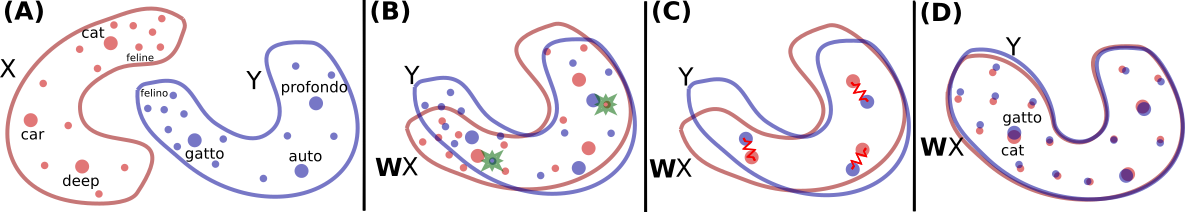
\includegraphics[width=0.8\textwidth]{vector_spaces_alignment.png}
  \caption{Aligning bilingual vector spaces. \parencite{Conneau:2017aa}}
  \label{fig:vec_space_align}
\end{figure}

In the multilingual scenario, alignment in two different vector spaces is vital in order to make word embeddings from different languages comparable. Figure \ref{fig:vec_space_align} illustrated the alignment method from \textcite{Conneau:2017aa}. Suppose there is a set of word pairs $\{x_i, y_i\}$ where ${i\in \{1, ..., n\}}$, the two vector spaces were aligned by a rotation matrix $W \in \mathbb{R}^{d \times d}$ as shown in process \textbf{(B)}, to optimize the objective function 

\begin{equation*}
  \min_{W \in \mathbb{R}^{d \times d}} \frac{1}{n}\sum_{i=1}^n \ell(Wx_i, y_i)
\end{equation*}

\noindent Here $\ell$ is the loss function and it is usually the square loss function $\ell(x, y)=||x-y||^2$. Then $W$ is further refined in process \textbf{(C)}, where we choose frequent words as anchor points and minimize the distance between each correspondent anchor points by an energy function. After this, the refined $W$ is then used to map all words in the dictionary during the inference process. We obtain the translation $t(i)$ of a given source word $i$ in the formula

\begin{equation*}
  t(i) = \argmin_{j\in \{1, ..., N\}} \ell(Wx_i, y_j)
\end{equation*}

Despite the mathematically proven theoretical feasibility, we need data to drive the alignment process. Lexicon is the most common form of such seed parallel data, though there are other kinds of alignment using data from sentence or documents \parencite{Ruder:2019aa}.

By using word-level information, we can start with a pivot language (usually English) and map each other monolingual word embeddings by looking the same word up in a dictionary \parencite{Mikolov:2013ac}. Sentence-level parallel data is similar to the role of corpora in Machine Translation (MT) since they both contain mapped sentences \parencite{Hermann:2013aa}. Document-level information is usually topic-aligned or class-aligned, such as data of the same Wikipedia item \parencite{vulic-moens-2013-study}.

Recent development in word alignment has showed possibilities for less supervision and smaller seed data size to initiate the alignment process \parencite{Ruder:2019aa}. Though it is still unclear if cross-lingual word embedding alignment can run without parallel data or supervison \parencite{Dyer1365879}, there are evidences that even distant language pairs have an accurate linear mapping \parencite{Mikolov:2013ac}. If such linear mapping does exist for every language in the word, and if it can be accquired through deep learning, people could build machine translation systems that are able to translate words in unseen languages.

\subsection{fastText}
\label{sec:fasttext}

In this work, we have chosen fastText aligned word vectors \parencite{Joulin:2018aa} as the vectorized word representation.\footnote{\url{https://fasttext.cc/docs/en/aligned-vectors.html}} They are based on the pre-trained monolingual vectors computed from the Wikipedia corpus using fastText \parencite{Bojanowski:2016aa}.

fastText is an extension of the original Word2Vec methods, which uses sub-words to augment low-frequency and unseen words. Take word \texttt{low-key} as an example. As a whole word, its possibility in a given document would be much lower than its components, \texttt{low} and \texttt{key}. fastText learns its vectorized representation from a smaller n-gram sub-word level. It divides the whole word \texttt{low-key} into sub-words units (assume $n=3$)

\begin{equation*}
  \mathtt{\text{<}lo, low, ow\text{-}, w\text{-}k, \text{-}ke, key, ey\text{>}}
\end{equation*}

\noindent Each sub-word has its own vectorized representation learned through a CBOW or Skip-gram model as in Word2Vec. The word vector for the whole word unit \texttt{<low-key>} is then the sum of all of its sub-word vectors. Hence its rareness would be compensated by two more frequent subwords \texttt{low} and \texttt{key}, even if it might not appear in the training document at all.

In addition to the advantage in representing rare words, fastText aligned word embeddings also has a large collection of embeddings for multiple languages, making it attractive to cross-lingual word embedding experiments. Thus fastText was selected in this thesis to save effort on training and alignemnt cross-lingual word embeddings, making it possible to concentrate more on experiments themselves.

\section{Multilingual Neural Machine Translation (NMT) Systems}

\subsection{Multilingual Neural Machine Translation}

Neural Machine Translation (NMT) uses neural networks to learn the translation relationship between a source and a target language. It has outperformed the traditional statistical machine translation in some machine translation settings and has enabled some new possibilities in the field. One of these new applications is multilingual Neural Machine Translation. As shown in Figure \ref{fig:google_mnmt}, the system has an encoder and a decoder consisting of several layers of LSTM network spread parallelly on multiple GPUs. An attention module serves as the connection bridge between the encoder and the decoder. It emphasizes which part of the source sentence is more relevant to the current translation context, especially when translating long sentences. \parencite{Wu:2016aa}. Multilingual NMT uses the same attentional encoder-decoder model but trains it on a multilingual corpus with additional artificial tokens to indicate the target language \parencite{Johnson:2016aa}.

The benefit of such a multilingual NMT system does not necessarily stop at higher translation performance between common languages like English, French, or Spanish; it also leverages additional information from high resource languages to low resource languages \parencite{Zoph:2016aa}. Such information leverage could be viewed as a special form of transfer learning \parencite{Zoph:2016aa}, which may happen both in the horizontal or vertical direction \parencite{Lakew:2019aa}: In the horizontal direction, knowledge transfers from pre-trained data (such as word embeddings or language models) to the raw test data; in the vertical direction, knowledge transfers from languages to languages, which could either transfer from high resource to low resource languages or from seen languages to unseen languages. The latter is called zero-shot translation.

\begin{figure}
  \centering
  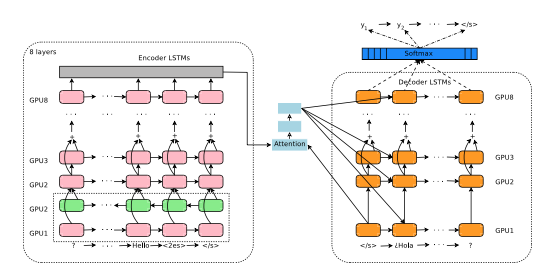
\includegraphics[width=0.8\textwidth]{google_mnmt_architecture.png}
  \caption{Google's MNMT Architecture \parencite{Johnson:2016aa,Wu:2016aa}}.
  \label{fig:google_mnmt}
\end{figure}

\subsection{Zero-shot Machine Translation}
\label{sec:zero_shot_mt}

Zero-shot translation stands for translation between language pairs invisible to the multilingual NMT system during the training time. For example, building a multilingual NMT system with German-English and French-English training language pairs while testing its performance on a German-French scenario. In 2016, \textcite{Johnson:2016aa} first published their result on a zero-shot MT system. Their multilingual MT system includes an encoder, a decoder, and an attention module. It requires no change to a standard NMT system except introducing an additional token at the beginning of each source sentence to denote the translation target language. \textcite{Ha:2016aa} also showed that their universal encoder and decoder model is capable of zero-shot MT. Translation between unseen language pairs is attractive, especially for low-resource language pairs. Compared with a pivot based system, zero-shot translation eliminates the need for a bridging language, or \textit{interlingua}, as an intermediary of the source and target language. However, zero-shot translation still underperforms than pivot-based translation.

Two reasons could explain the gap between a zero-shot system and a pivot based system, language bias \parencite{Ha:2016aa, Ha:2017aa, Arivazhagan:2019aa} and poor generalization \parencite{Arivazhagan:2019aa}. Language bias means that the MT system tends to decode the target sentence into the wrong language during inference, usually copying the source language or the bridging language \parencite{Ha:2016aa}. It could be the consequence of always translating all source languages into the bridging language, making the model difficult to learn to translate to the desired target language \parencite{Arivazhagan:2019aa}.

The other potential reason for the worse performance of a zero-shot system is poor generalization. When a zero-shot system is trained purely on the end-to-end translation objective, the model prefers to overfit the supervised translation direction features than learn more transferable language features. There is no guarantee that the model would discover language invariant representations as there is no explicit incentive to learn language invariant features, resulting in the intermediate encoder representations are too specific to individual languages \parencite{Arivazhagan:2019aa}.

To fix these two problems, there has been work on improving the preprocessing process \parencite{Lakew:2018aa}, parameter sharing \parencite{Firat:2016aa, Blackwood:2018aa}, additional loss penalty functions \parencite{Arivazhagan:2019aa} and pre-training modules using external information \parencite{Baziotis:2020aa}. In some of the improvements, zero-shot system could achieve better performance than pivot based systems.

\section{Cross-lingual Word Embeddings in Multilingual NMT}

In terms of the application of cross-lingual word embeddings in a multilingual NMT system, there are some successful applications such as using the cross-lingual word embeddings as the embedding layer \parencite{neishi-etal-2017-bag, Artetxe:2017aa}, as the substitution of a supervised dictionary \parencite{Conneau:2017aa}, or as an external supplementary extension \parencite{inproceedings}. There are even cases where people successfully trained an MT system using very little or none parallel data \parencite{Conneau:2017aa} and heavily rely on cross-lingual word embeddings. Nevertheless, in most MT systems, using pre-trained word embeddings purely as the embedding layer will not outperform other models such as Transformers \parencite{Vaswani:2017aa} and its other evolutions, largely because the training data for an MT system is usually several orders of magnitude larger than the monolingual pre-trained word embeddings.

\chapter{The Transferability of Multilingual NMT models to Unknown Languages}
\label{chap:research_question}

For NMT systems focused on low resource language, \textcite{Qi:2018aa} looked into when and why pre-trained word embeddings are useful. They found that pre-trained word embeddings are consistently useful for all languages. The gains would be more visible if the source and target language are similar, such as languages within the same family. \textcite{Qi:2018aa} also looked at aligned pre-trained word embeddings and their performance in a multilingual setting. They found that aligned pre-trained word embeddings are useful in a multilingual NMT system, while in bilingual NMT systems, pre-trained word embeddings do not necessarily need to be aligned. \textcite{Qi:2018aa} attributed the BLEU score increase to the architecture of an attentional encoder-decoder multilingual NMT system. As such multilingual NMT system uses a single encoder for all source languages, alignment in the word embeddings concentrates various vector spaces of the source language into a unified vector space, helping the system learn a much-simplified transform from its input vector space to its output vector space.

In conclusion, cross-lingual word embeddings appear to be a good enhancement to multilingual NMT systems, especially for systems specialized for translating low-resource languages. However, most of the previous application of cross-lingual word embeddings target zero-shot language pairs, not on completely unseen languages. They examed their results on test sets whose language in both the source or target side of the translation is known to the system, but their paired combination remains unknown. For language pairs $A \rightarrow \text{EN}$ and $\text{EN} \rightarrow B$, they are all interested in the unseen language pair $A \rightarrow B$. For language pairs that include an unseen language $C$, whether on the source side or the target side, it remains to see how cross-lingual word embeddings could help translate in this scenario.

In this work, we would like to take a step further to see how multilingual NMT systems with cross-lingual word embeddings would work for zero-resource languages --- languages that are entirely unseen to the multilingual NMT setting. We would like to examine the transferability of multilingual NMT models to an unknown language. The transferability of multilingual NMT models is vital from both the theoretical and practical perspectives. The theoretical importance of these models come to the way that they find the correspondence between language pairs \parencite{Johnson:2016aa,lu-etal-2018-neural}. The practical importance is their effective use for the translation of low-resource languages \parencite{Zoph:2016aa,Nguyen:2017aa}.

As mentioned in Section \ref{sec:multilingual_word_embeddings}, \textcite{Mikolov:2013ac} showed that there is a linear relationship between similar word embeddings in different languages. Hence suppose we have the input and the output word vector space, there will be a linear relationship between these two vector spaces. The output vector space $Z_\text{out}$ could be a sementic space from one of the known languages, but what we are interested in is to see if such linear mapping still holds when we change the output vector space to an unknown sementic space from an unseen language.

We define of our research question as follows. Given a vector space $Z$ that consists of cross-lingual word embeddings and a transform matrix $W$ that approximates vectors $X$ from the input vector space $Z_\text{in}$ to vectors $Y$ from the output vector space $Z_\text{out}$, we want to test if the equation

\begin{equation*}
  Y^\prime = \sum_{i=0}^n WX_i
\end{equation*}

\noindent is still true. Here $Y^\prime$ is the vector from a new unknown vector space $Z_\text{unknown}$ but both $Z_\text{in}$, $Z_\text{out}$ and $Z_\text{unknown}$ are aligned.

\chapter{Methodalogy}
\label{chap:method}

In this chapter, we will perform experiments in a cross-lingual word embedding based multilingual NMT system to see the transferability of the model on the test languages.

\section{Experiment Settings}
\label{sec:initial_exp_settings}

We chose English (EN), German (De), and French (FR) to be the training languages as these three romance languages are all considered to be high-resource languages. Furthermore, \textcite{Qi:2018aa} observed that pre-trained word embeddings are useful for languages from the same language family. The closer their relationship is, the higher the performance improvement is. Since language similarity plays a role in the multilingual NMT system performance, these three languages are related to many other Indo-European languages. Selecting them as our training languages would enable a wider choice of testing languages later on in the experiments.

Let $C$ donate the final corpus, $l$ donates the language-specific corpus fragment and $Z$ is the set of corresponding candidate languages, the training language set is then $Z_{TRAIN} = {l_{EN}\cup l_{DE}\cup l_{FR}}$. For the test language set, we picked up Swedish (SV), Hungarian (HU), and Hebrew (HE) as three low-resource language representations within the same langauge family of our training languages. Therefore $Z_{TEST} = {l_{SV}\cup l_{HU}\cup l_{HE}}$.

For each experiment, we trained a basic multilingual NMT system using a training corpus $C_{TRAIN}$ with all three training languages, including all six directions from the cartesian product without duplicates. Here $x$ and $y$ are both training languages in the training set $C_{\text{TRAIN}}$.

\begin{equation*}
  C_{\text{TRAIN}} = \{x \times y \mid x, y \in Z_{\text{TRAIN}} \text{ and } x \neq y\}
\end{equation*}

During testing, the multilingual NMT system is tested on the test corpus with all three training languages and one of the test language. The test corpus consists of both translation directions of three different training language and that only test language.

\begin{equation*}
  C_{\text{TEST}} = \{(x, y)\cup(y,x) \mid x \in Z_{\text{TRAIN}} \text{ and } y \in Z_{\text{TEST}}\}
\end{equation*}

\subsection{Corpus and Preprocessing}

we have used the TED talk subtitle corpus from \textcite{Qi:2018aa} \footnote{\url{https://github.com/neulab/word-embeddings-for-nmt}} to train the multilingual NMT. The whole corpus has roughly $\num{2.7e6}$ sentences split into three parts, train, dev, test at the ratio of $0.95:0.025:0.025$.

To build up the corpus for each experiment, the author has modified the original script from \textcite{Qi:2018aa} and added a few customized features. In short, the script will extract shared sentences from each part of the split corpus to form up a common intersection used in training, developing, and testing. Since the experiments consist of languages that are relatively common in the TED project, this fine-tuned corpus is not too different from the original corpus, hence after all the sizes for the train, dev, and test split were kept.

For preprocessing, since the original TED corpus is already tokenized by Moses, we did not add additional tokenization steps. We turned all of the text into lower cases and applied a sentence length filter to remove any long sentences with more than 60 words. The sentence length filter prevents inferior performance in training. After that, when building the index to word (i2w) and the word to index (w2i) table for the pre-trained embeddings. We have also removed any words that are less frequent than two times to stop the system from overfitting by low-frequency words. All of the preprocess functions are built upon the built-in XNMT preprocess features \parencite{Neubig:2018aa}.

\subsection{Neural Network}

The neural network is a modified version of the one from \textcite{Qi:2018aa}, which is built with XNMT \textcite{Neubig:2018aa}. The only change is doubling the encoding layer to a 2-layer-bidirectional LSTM network, thus having more parameters to accommodate the additional information in a multilingual scenario. Everything else is the same as the original experiment settings, see Table \ref{table:hyperparameters}. We use BLEU score \parencite{papineni-etal-2002-bleu} as well as 1-4gram precison scores as our evaluation metrics. The initial learning starts at $0.0002$ and decays by $0.5$ when development BLEU score decreases \parencite{Denkowski:2017aa}.

\begin{table}
  \centering
  \begin{tabular}{|r|l|}
    \hline
    Hyperparameter & Value \\ [0.25ex]
    \hline\hline
    Beam size & 5 \\
    \hline
    Batch size & 32 \\ 
    \hline
    Dropout & 0.1 \\
    \hline
    Optimizer & Adam \parencite{Kingma:2014aa} \\
    \hline
  \end{tabular}
  \caption{Hyperparameter settings)}
  \label{table:hyperparameters}
\end{table}

\subsection{Embeddings}

The embeddings used in the experiments are fastText aligned word embeddings\footnote{\url{https://fasttext.cc/docs/en/aligned-vectors.html}}. They are based on the pre-trained vectors on Wikipedia\footnote{\url{https://www.wikipedia.org/}} using fastText \parencite{Bojanowski:2016aa}. The alignment is performed using RCSLS as in \textcite{Joulin:2018aa}.

Each of the fastText word embedding file is language-specific and contains word embeddings in 300 dimensions. We concatenated different language files to build up cross-lingual word embedding files for the multilingual NMT system. The embeddings are forzen during the whole training so that they will remain the original alignment throught out the whole experiment. If there is a shared word with two different vector values in different language embedding files, the average value of both vectors will be used.

In this way, there are possibilities that both of the unique semantic values in the two words $w_a$ and $w_b$ could be lost, as there are cases that word with distant meaning share the same spelling in different languages. However, people could also argue that many words with the same spelling do have a similar meaning. For example, the word \verb|café| means the same thing in English and French, as English borrowed that word from French. Later in the experiment, there will also be a different attempt where the system treats each word as a unique word even though they might share the same spelling. Both of the results will be available below in Section \ref{sec:results_source_and_target_annotation}.


\chapter{Results and Analysis}
\label{chap:results}

\begin{table}
  \centering
  \begin{tabular}{|r*{5}{|l}|}
    \hline
    Language & BLEU & 1gram & 2gram & 3gram & 4gram \\ [0.25ex]
    \hline\hline
    EN+DE+FR & 29.22 & 0.57 & 0.34 & 0.24 & 0.16 \\
    \hline
    SV & 1.12 & 0.16 & 0.02 & 0.00 & 0.00 \\ 
    \hline
    HU & 1.12 & 0.18 & 0.02 & 0.00 & 0.00 \\
    \hline
    HE & 1.02 & 0.16 & 0.02 & 0.00 & 0.00 \\
    \hline
  \end{tabular}
  \caption{Initial results for SV, HU and HE on the baseline system (Target language annotation only, dropout=0.3, trained on mixed language branch corpus.)}
  \label{table:initial_results}
\end{table}

In the results shown in Table \ref{table:initial_results}, Swedish, Hungarian and Hebrew all got unanticipated low BLEU scores. Even though Swedish is closer to the training languages, the expected high perfromance from Swedish did not appear in the experiment result. All of the three languages only achieved around 1 BLEU score. Also, since the system hardly translates any of the languages (as examples in \ref{sec:initial_output}), it is hard to tell the relationship between language similarity and the model's performance. However, when it comes to random initialized embedding layers without pre-trained embeddings, cross-lingual word embeddings still provides better initialization than nothing. We see the translation model trained with cross-lingual embeddings performs substantially better (Avg BLEU=1.2) than a model trained with random initialized embeddings (BLEU=0.1).

By looking at individual 1-4 gram precision scores, all three languages had a significantly better unigram precision score than their bigram, trigram, and quadgram precision score. For example in Swedish its bigram precision score in Swedish was about half of its unigram scores. The precison score on trigrams and quadgrams are close to 0 on all languages, which again is a sign showing the multilingual NMT system has little transferability from known training languages to an unknown test language, and that transferability only happens at word level.

We have tried increasing the dropout rate to 0.3 in order to transfer more information from known languages to unknown languages, but we only observed small improvements (average 0.5 BLEU score increase). Since this technique improves the zero-shot performance at the cost of supervised translation directions \textcite{Arivazhagan:2019aa}, we decided to explore other approaches in below.

\section{The Effect of Source/Target Language Annotation}
\label{sec:results_source_and_target_annotation}

Inspired by \textcite{Blackwood:2018aa}, the first improvement is to alter the way the target language annotation in the source sentences. In the original corpus building script, it will add a custom \verb|__{lang_id}__| token at the front of each source sentence, as suggested by \textcite{Johnson:2016aa}. A sentence in the annotated source text whose target language is German would look like 

\begin{verbatim}
  __de__ and we struggle with how to deal with them .
\end{verbatim}

Later two other tokens --- a single source token and a source token together with a target token, were added into the experiments. Hence a sentence in English would look like this. 

\begin{verbatim}
  __en__ and we struggle with how to deal with them .
\end{verbatim}

When it needs to be translated into German, the annotation would then become 

\begin{verbatim}
  __en__ __de__ and we struggle with how to deal with them .
\end{verbatim}

\begin{table}
  \centering
  \begin{tabular}{|r*{3}{|l}|}
  \hline
  Languages & TGT & SRC & Full \\
  \hline\hline
  EN+DE+FR & 29.22 & 17.59 & 28.73 \\
  \hline
  SV & 1.12 & 0.00 & 1.16 \\
  \hline
  HU & 1.12 & 0.00 & 1.12 \\
  \hline
  HE & 1.02 & 0.00 & 1.02 \\
  \hline
  \end{tabular}
  \caption{BLEU scores for different language annotations (Target only, source only and full annotation)}
  \label{table:altering_lang_id}
\end{table}

The results are in Table \ref{table:altering_lang_id}. Adding a source token together with the target token did not change the overall result much, but removing the target token had a negative impact on the final BLEU score. This observation is in line with previous claims and results \parencite{Johnson:2016aa, Blackwood:2018aa} that the multilingual NMT system requires a target token at the beginning of each sentence to help identify the target language.

Compared with \textcite{Blackwood:2018aa}, our experiments with altered language annotation did not improved the model's transferability to unknown languages. Even though our target specified annotation also yields the best results, the multilingual NMT model still can not learn to output the correct language since the desired target token remains unseen to the system. Altering target token annotation is not effective in our experiments.

\section{The Effect of Language Similarity}
\label{sec:langauge_similarity}

To deeper undetstand how and why Swedish benefited from its language similarity to our training languages, we have further designed experiments to see the effect of language similarity.

The additional experiments will still use Swedish as the test langauge while remove French as the training language to homogenize the training language set more towards Swedish. In the previous training language set, French is the only training language that is Romanic. By replacing French with Danish, all of the training languages are now Germanic, as well as the test language Swedish. We have also included two more Germanic languages to the training language set, Dutch (NL) and Norwegian (NO). We began with an experiment trained on English, German and Danish, and added the additional training languages one by one in the next two expriments. Everything else is the same. The results are shown in Table \ref{table:language_similarity}.

\begin{table}
  \centering
  \begin{tabular}{|r*{5}{|l}|}
  \hline
  Language & BLEU & 1gram & 2gram & 3gram & 4gram \\ [0.25ex]
  \hline\hline
  EN+DE+FR & 1.12 & 0.16 & 0.02 & 0.00 & 0.00 \\
  \hline
  EN+DE+DA & 4.1 & 0.28 & 0.07 & 0.02 & 0.01 \\
  \hline
  +NL & 3.3 & 0.23 & 0.05 & 0.02 & 0.00 \\ 
  \hline
  +NO & 4.7 & 0.31 & 0.07 & 0.03 & 0.01 \\
  \hline
  \end{tabular}
  \caption{Results for language similarity tested on the Swedish language. Three other Germanic languages DA, NL and NO were added one by one into the training corpus.}
  \label{table:language_similarity}
\end{table}

As the results shows, the system gained most improvements when Danish and Norwegian were added. Despite Dutch and Swedish are both Germanic languages, Dutch does not help the multilingual NMT system to learn how to translate from Swedish or into Swedish a lot. This confirms that close languages would benefit each other more than distant languages in a multilingual NMT systemn using pre-trained word embeddings \parencite{Qi:2018aa}.

Swedish, Danish and Norwegian have deep historical relationships to each other. As a result, these languages share many vocabularies as well as grammar and syntax rules. To study how much of such kind of benefit were brought by shared vocabluaries or their similar syntax, each word in the training corpus was tagged by its source language token to distinguish its origins. Punctuations are not distinguished among languages, which means they don't receive a language-specific token. The word embeddings also tagged to point it to the correct source word. A Swedish sentence that needs to be translated into German is then 

\begin{verbatim}
  __de__ <<sv>>och <<sv>>vi <<sv>>kämpar <<sv>>med <<sv>>dem .
\end{verbatim}

The assumption behind the word origin token is that, if the result suffers when each word differs by its origin language, the multilingual NMT system would primarily translate by shared vocabularies between language; if its results still holds after the modificaiton, it would primarily learn translation from shared syntax information instead.

The system has obtained 1.7 BLEU score on the EN+DE+DA to SV experiment. It showed that if each word is no longer allowed to be shared between languages the models's performance would dramatically decrease, hence most of the improvements were brought by the fact that Swedish, Danish and Norwegian have a large amount of common vocabluaries. On the other side, it also indicates that the system didn't learn too much syntactic information during training. Even though these languages have similar grammar structures, the system didn't catch it very well, otherwise we would see smaller BLEU score gap between the results as the close grammar relationship will be preserved in the embedding layer. The multilingual NMT system here primarily learns lexicon translation.

\section{The Effect of the Transformed Vector Space}

In addition to the role of language similarity between the training languages and the test languages, we also hypothesis that the poor transferability of our multilingual NMT model to unseen languages is due to transformed vector space in the translation model. After a series of linear opeartion from the neural network onto the word embeddings, the output vector space is no longer aligned with the input vector space. This is based on the hypothesis that our NMT system have already learned the genrally mapping between words in the source vector space and the ones in the target vector space, even though the correct word in the target word space hasn't been seen by the system during training. However since every cross-lingual word embeddings are grouped by their semantics, the correct target word should also be around the wrong output word.

By looking closely from the predicted translation in Table \ref{table:initial_results}, we have observed the contrary --- almost none of the words in the output text is translated to the correct word in the desired languages. They were either translated into one of the training languages, or were entirely copied from the source text. The BLEU score gains were from punctuations and a small collection of words shared between languages (e.g. property nouns).

Taking a step further, when analyzing both translation directions there are other traces to support our transformed vector space hypothesis. We have conducted comparisions on both directions on the Swedish language experiment, as shown in Table \ref{table:directional_results}. When tranlsating from SV to the combined EN+DE+DA text, we could achieve almost 6 BLEU scores, which is much better than the nearly zero score when translating from the other direction. Also compared to the combined precision scores on the same experiment from Table \ref{table:language_similarity}, the results of the translation direction EN+DE+DA $\rightarrow$ SV contributed almost nothing to the combined translation performance.  We present the sample output of both directions in Appendix \ref{sec:directional_output}.

\begin{table}
  \centering
  \begin{tabular}{|r*{5}{|l}|}
  \hline
  Language & BLEU & 1gram & 2gram & 3gram & 4gram \\ [0.25ex]
  \hline\hline
  EN+DE+DA $\rightarrow$ SV & 0.65 & 0.14 & 0.01 & 0.00 & 0.00 \\
  \hline
  SV $\rightarrow$ EN+DE+DA & 6.00 & 0.33 & 0.08 & 0.03 & 0.01 \\
  \hline
  \end{tabular}
  \caption{Results for individual translation direction between EN+DE+DA and SV.}
  \label{table:directional_results}
\end{table}

Thus, it is highly possible to suspect the output vectors from the model's decoder have been altered and are no longer in the same vector space as the input word embeddings. In this case, the transformed vector space has also made less sense to search for the correct word vector neighbours close to the predicted ouput vector in the output vector space. However, there opens a new possible to translate from completely unknown languages to known languages. We could perform a lexicon replacement based on the Euclidean distance between words in the unknown language and one of the known languages, then feed the processed text into a translation model which has already been trained on known languages. During the whole process, the unknown langauge remains untouched by the translation model hence it still qualifies as zero-resource translation. We will discuss the lexicon replacement process below.

\subsection{Lexicon Replacement By Euclidean Distance}

Suppose we have a vector space $S$ that contains cross-lingual word embeddings in the unknown language and the known languages, respectively. We donate them as $W_x$ and $W_k$. For each $w_x\in W_x$, there exists at least one mapping to a target word in the known languages $w_k \in W_k$. We are looking for that specific $w_k$ that are with in a specific radius of the original $w_s$. The distance should still be relatively small so that $w_s$ and $w_k$ are both considered to be an effective translation of each other.

In theory, to determine the nearyby neighbour $w_k$, we can use different kinds of metrics. Here we have chosen to use the Euclidean distance where determines the distance between $w_s$ and $w_k$ as

\begin{equation}
  d(w_s, w_k)=\sqrt{\sum_{i=1}^n{(w_{s_i}-w_{k_i})}^2}
\end{equation}

The distance $d$ is a variable here and its value needs to be determined as well. Hence there are experiments to test the distance argument $d$ by different experiments, ranging from $d=0.25$ to $d=5$.

The algorithm is described in Algorithm \ref{algo:subsitution}.

\begin{algorithm}[h]
  \SetAlgoLined
  \KwIn{hypothesis $H$, source language embeddings $E_s$, target language embeddings $E_t$, distance threshold $D$}
  \KwResult{Updated hypothesis $H^\prime$ with words being replaced by their neighbors in the desired language}

  Build kd-tree $T$ from $E_s$
  \For(each line $l$ in the source hypothesis $H$){$l \in H$}{
    \For(each word $w$ in line $l$){$w \in l$}{
      \uIf{$w$ is a punctuation}{
        skip $w$\;
      }
      \uElseIf{$w$ is an unknown word}{
        skip $w$\;
      }
      \Else{
        query distance $d(w, w^\prime)$ for $w$ in $T$\;
        \If{$d<D$}{
          replace $w$ with the correspoding $w^\prime$
        }
      }
    }
  }
  \caption{Pesudo code for output hypothesis word subsitution. Each word in the NMT output hypothesis that are not in the desired language will be replaced by its cloeset neighbour in that language.}
  \label{algo:subsitution}
\end{algorithm}

Performing a distance query on a vector space that has more than $\num{3e6}$ vectors is slow, especially when all these vectors are considered to be high dimensional vectors. The code was implemented with SciPy \parencite{Virtanen:2019aa}. There are algothrims like KD-tree \parencite{Maneewongvatana:aa} that could reduce the calcualtion time for low-dimensional vectors, but for vectors that are higher than 20 dimentions it is not necessarily faster than brutal force.\footnote{As descibed on the API document, "High-dimensional nearest-neighbor queries are a substantial open problem in computer science.", \url{https://docs.scipy.org/doc/scipy/reference/generated/scipy.spatial.KDTree.html}} On the other hand, based on the Johnson–Lindenstrauss theorem \parencite{johnson1984extensions}, a vector space should have at least more than 300 dimensions to distinguish $\num{1e6}$ vectors in it. As the aligned vector space in fastText contains more than $\num{3e6}$ words, the dimensions could not be compressed any more or you are at risk of not be able to distinguish each word. All in all, the script is slow at subsitute every word in the output hypothesis into the correspoding one in the desired language.

We have performed the lexicon replacement experiment on the SV $\leftrightarrow$ EN+DE+DA text from the same TED text corpus \parencite{Qi:2018aa}, feeded into an already trained tranlsation model based on the NO $\leftrightarrow$ EN+DE+DA corpus, using NO as the pivot language. When applying the previously mention Algorithm \ref{algo:subsitution} on the SV $\leftrightarrow$ EN+DE+DA text, we replace all of the source text started without the target langauge token \verb|__SV__|. In other words, we translate all of the source sentence in Swedish to Norwegian first, leaving all of the other source sentences (sentences in EN, DE or DA) untouched. The target translation reference is also remained as is. 

The BLEU scores are shown in Table \ref{table:lexicon_replacement}. In order to demostate the difference of applying the same algorithm on the input and the output vector space, we have also selected result from $d=0$ to $d=4$ and compared them with the results when Algorithm \ref{algo:subsitution} was performed on the output vector space. The comparision is in Figure \ref{fig:lexicon_replacement}.

\begin{table}
  \centering
  \begin{tabular}{|r*{5}{|l}|}
  \hline
  $d$ value & BLEU & 1gram & 2gram & 3gram & 4gram \\ [0.25ex]
  \hline\hline
  SV $\leftrightarrow$ EN+DE+DA & 4.1 & 0.28 & 0.07 & 0.02 & 0.01 \\
  \hline
  No replacement & 2.99 & 0.27 & 0.05 & 0.02 & 0.00 \\
  \hline
  0.25 & 2.99 & 0.27 & 0.05 & 0.02 & 0.00 \\
  \hline
  0.5 & 2.99 & 0.27 & 0.05 & 0.02 & 0.00 \\
  \hline
  1 & 6.18 & 0.34 & 0.10 & 0.04 & 0.01 \\
  \hline
  2 & 6.17 & 0.34 & 0.10 & 0.04 & 0.01 \\
  \hline
  3 & 6.17 & 0.34 & 0.10 & 0.04 & 0.01 \\
  \hline
  4 & 6.17 & 0.34 & 0.10 & 0.04 & 0.01 \\
  \hline
  0 & 6.00 & 0.33 & 0.08 & 0.03 & 0.01 \\
  \hline
  \end{tabular}
  \caption{Results for the lexicon replacement experiments with different $d$ thresholds. Tested on SV text using NO as the pivot language on the NO $\leftrightarrow$ EN+DE+DA translation model. $d=0$ stands for no threshold control (replace every word).}
  \label{table:lexicon_replacement}
\end{table}

\begin{figure}
  \centering
  \resizebox{0.7\columnwidth}{!}{%
      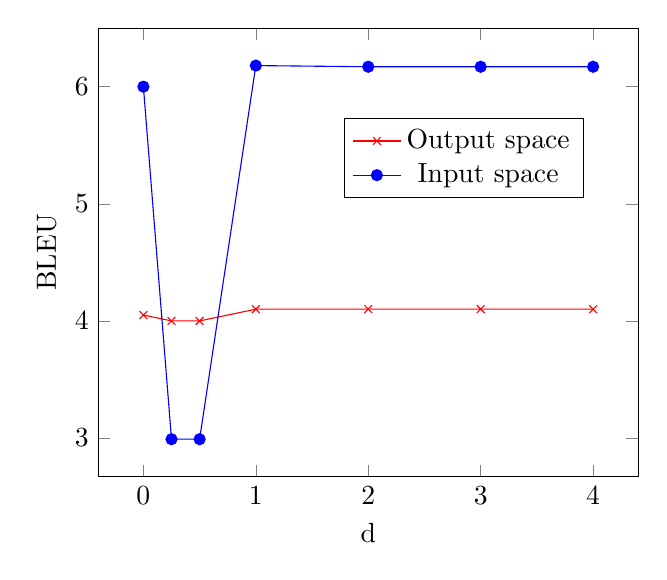
\begin{tikzpicture}
        \pgfplotsset{
          every axis legend/.append style={
            at={(0.9,0.8)},
            anchor=north east,
          },
        }
        \begin{axis}[
          xlabel=d,
          ylabel=BLEU]
        \addplot[color=red,mark=x] coordinates {
          (0,4.05)
          (0.25,4.0)
          (0.5,4.0)
          (1,4.1)
          (2,4.1)
          (3,4.1)
          (4,4.1)
        };
        \addplot[color=blue,mark=*] coordinates {
          (0,6.00)
          (0.25,2.99)
          (0.5,2.99)
          (1,6.18)
          (2,6.17)
          (3,6.17)
          (4,6.17)
        };
        \legend{Output space, Input space}
        \end{axis}
      \end{tikzpicture}
  }
  \caption{BLEU scores for the lexicon replacement algorithm applied on both the input and the output vector space.}
  \label{fig:lexicon_replacement}
\end{figure}

From both Table \ref{table:lexicon_replacement} and Figure \ref{fig:lexicon_replacement}, we can see a noticeable improvement over the baseline result as the BLEU score doubled. Even compared with the SV $\leftrightarrow$ EN+DE+DA model, the result from the lexicon replacement experiment is still leading ahead for about 2 BLEU scores. Thus it demostrates that our lexicon replacement hypothesis is effective within the input vector space.

Moreover, the value $d$ will affect the translation model. As we increase $d$ from $0.5$ to $1$ we see a big tranlation quality improvement. On the other side, increasing $d$ after $d=1$ will have no positive impact on the model's performance. When we set $d=0$ to remove the threshold control its performance even dropped around $0.2$ points, mostly due to the lowered bigram precison score. We conclude that there is a sweet spot for the $d$ value, though its accurate value needs to be fine tuned to adapt different source and pivot language combinations.

Finally, when comparing the results of lexicon replacement on the input vector space and the results on the output vector space, we confirmed the output vector space did changed during the translation tranining process by the model's neural network. Unlike the input vector space, excuting lexicon replacement on the output space does not have a leap on the BLEU score no matter how the distance threshold $d$ changes. Hence it is not worth to perform operations like lexicon replacement on the output vector space.

\chapter{Conclusion and Future Work}
\label{chap:conclusion}

In this thesis, we have explored the transferring and generalizability of cross-lingual word embeddings on unknown languages. From the achievement of zero-shot machine translation, we took a step further and expected moderate performance from those word embeddings as if they would transfer knowledge learned from the test languages onto other completely unknown languages. However, our experiment results suggested that only slight knowledge transfer happened between closely related languages, which echoes back to some of the findings that the embedding layer along in a multilingual NMT system is not enough to handle the knowledge transfer \parencite{aji-etal-2020-neural}.

To increase cross-lingual word embeddings' transferability in a multilingual NMT architecture similar to \textcite{Johnson:2016aa}, there should be some additional alignment in the output vector space between the source and the target languages. During the training process, the neural network has never seen any positive examples from the test language. Therefore its output weight on the test language has been continuously deducted, which resulted in a transformed output vector space. Such output space is no longer aligned with the input vector space, hence connections between different languages solely rely on shared vocabularies. As a result, only very similar languages such as Swedish, Norwegian and Danish benefited in our experiments.

As we have demonstrated in our lexicon replacement experiments, a solution to align the deviated input and output embedding spaces is to add regularization to the multilingual model's loss function base on the divergence of the two vector spaces. Another potential solution to be explored is to supplement the translation model with language level information such as language embeddings \parencite{littell-etal-2017-uriel,malaviya-etal-2017-learning} together with the cross-lingual embeddings. Language level information could also answer more questions remained in our study. Together with some previous studies \parencite{Qi:2018aa,aji-etal-2020-neural}, we believe the transferability of cross-lingual word embeddings is related to the similarity between the source and the target language, but how to measure the language similarity and link it to the transferability of the embedding layers could be an exciting topic.

Finally, it is worth exploring how other sets of embeddings would enhance the transferability of cross-lingual word embeddings. For example, to try the multilingual contextualized cross-lingual embeddings \textcite{devlin-etal-2019-bert} and see if it would benefit the transferability by adding contextual information, or the multilingual sub-word embeddings \textcite{Heinzerling:2017aa} if it would perform better by aligning more words between different languages.

\appendix
\chapter{Example Output from the Multilingual NMT Model}
\label{chap:example_output}

\section{Example Output from the Initial Experiment}
\label{sec:initial_output}

This sample output is taken from the SV $\leftrightarrow$ EN+DE+FR experiment, described in Section \ref{sec:initial_exp_settings}. Its perfromance result is in Table \ref{table:initial_results}.

We haved sampled 20 sentences from the output file. Each of the languages (SV, EN, DE and FR) as the target translation langauge has 5 examples.

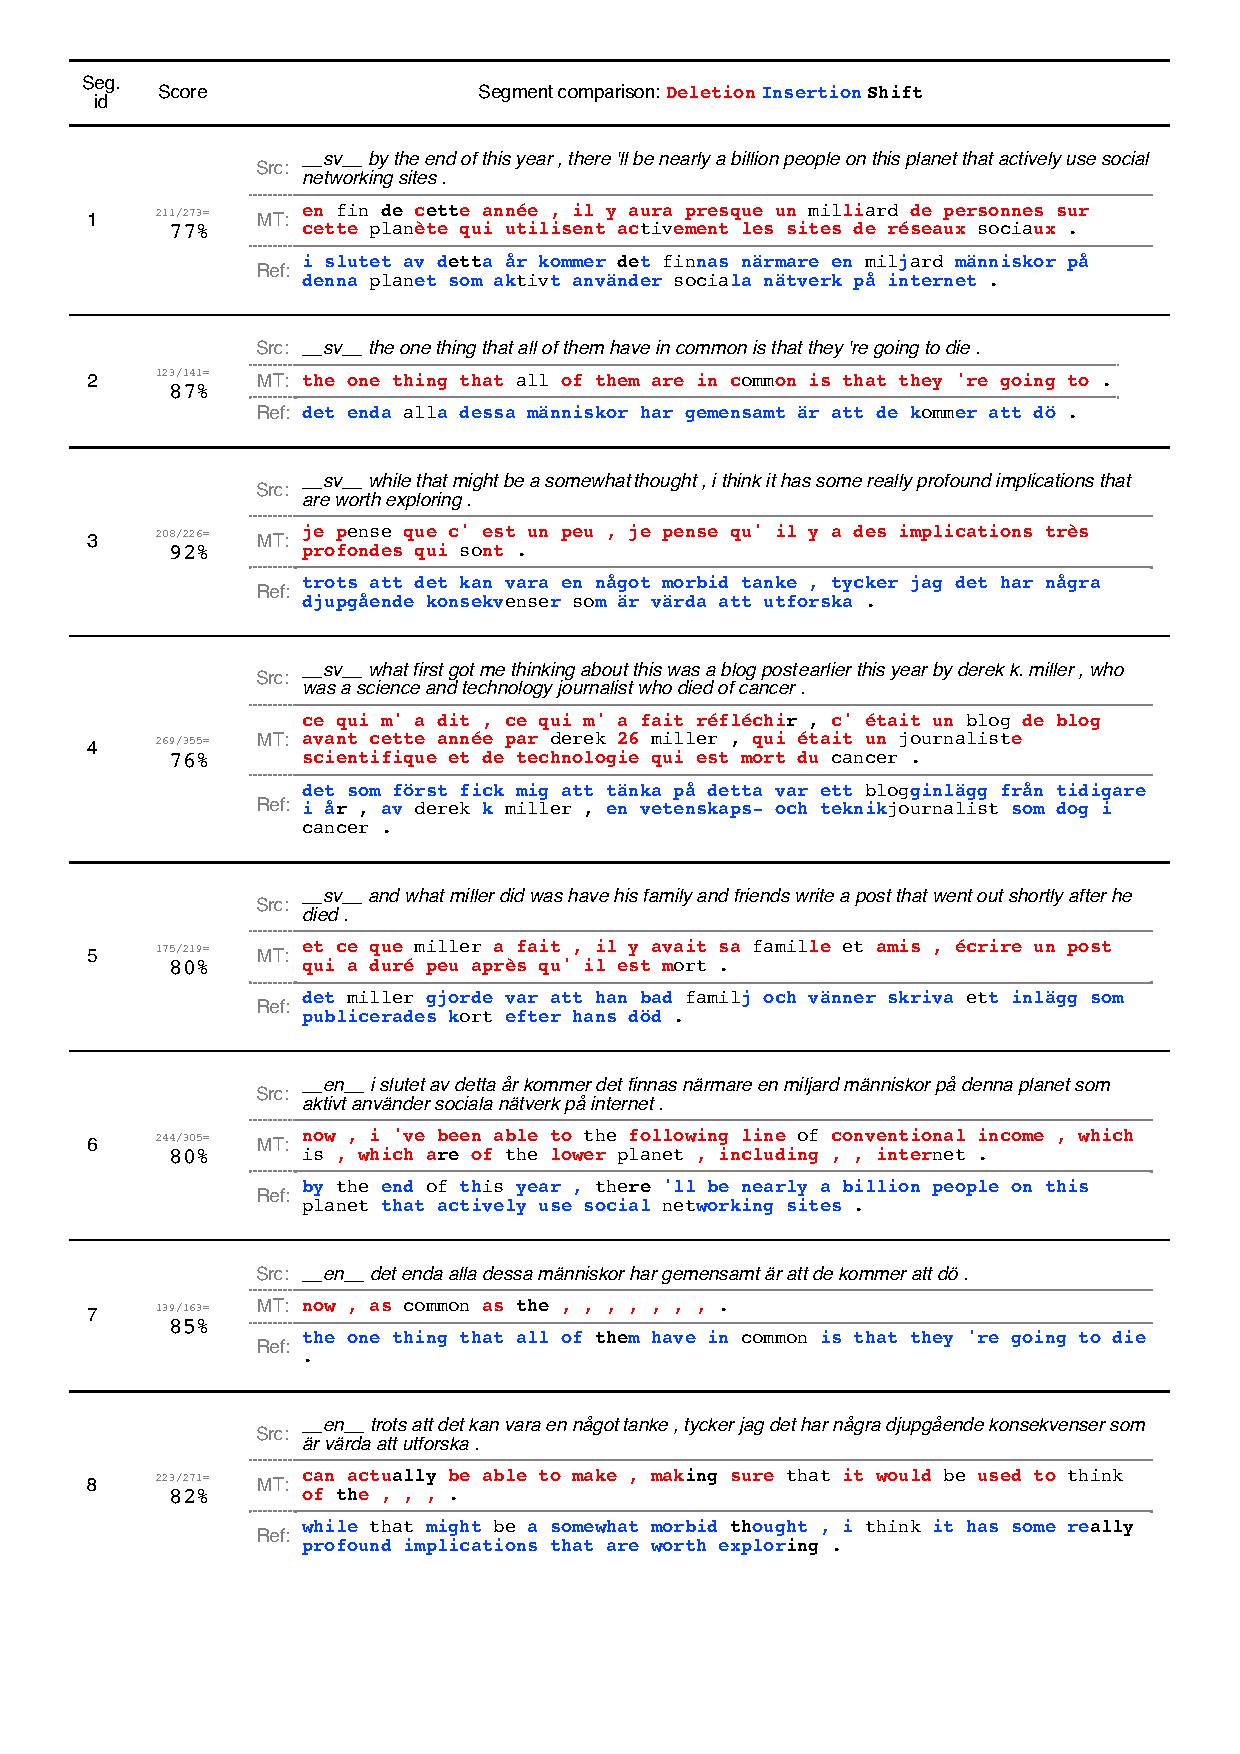
\includepdf[pages=-,scale=0.9,pagecommand={}]{mt_example_output/en+de+fr+sv.pdf}

\section{Example Output from the Directional Translation Experiment}
\label{sec:directional_output}

This sample output is taken from the SV $\leftrightarrow$ EN+DE+DA experiment, described in Section \ref{sec:langauge_similarity}. Its perfromance result is in Table \ref{table:language_similarity}.

We haved sampled 20 sentences from the output file. Each of the languages (SV, EN, DE and DA) as the target translation langauge has 5 examples.

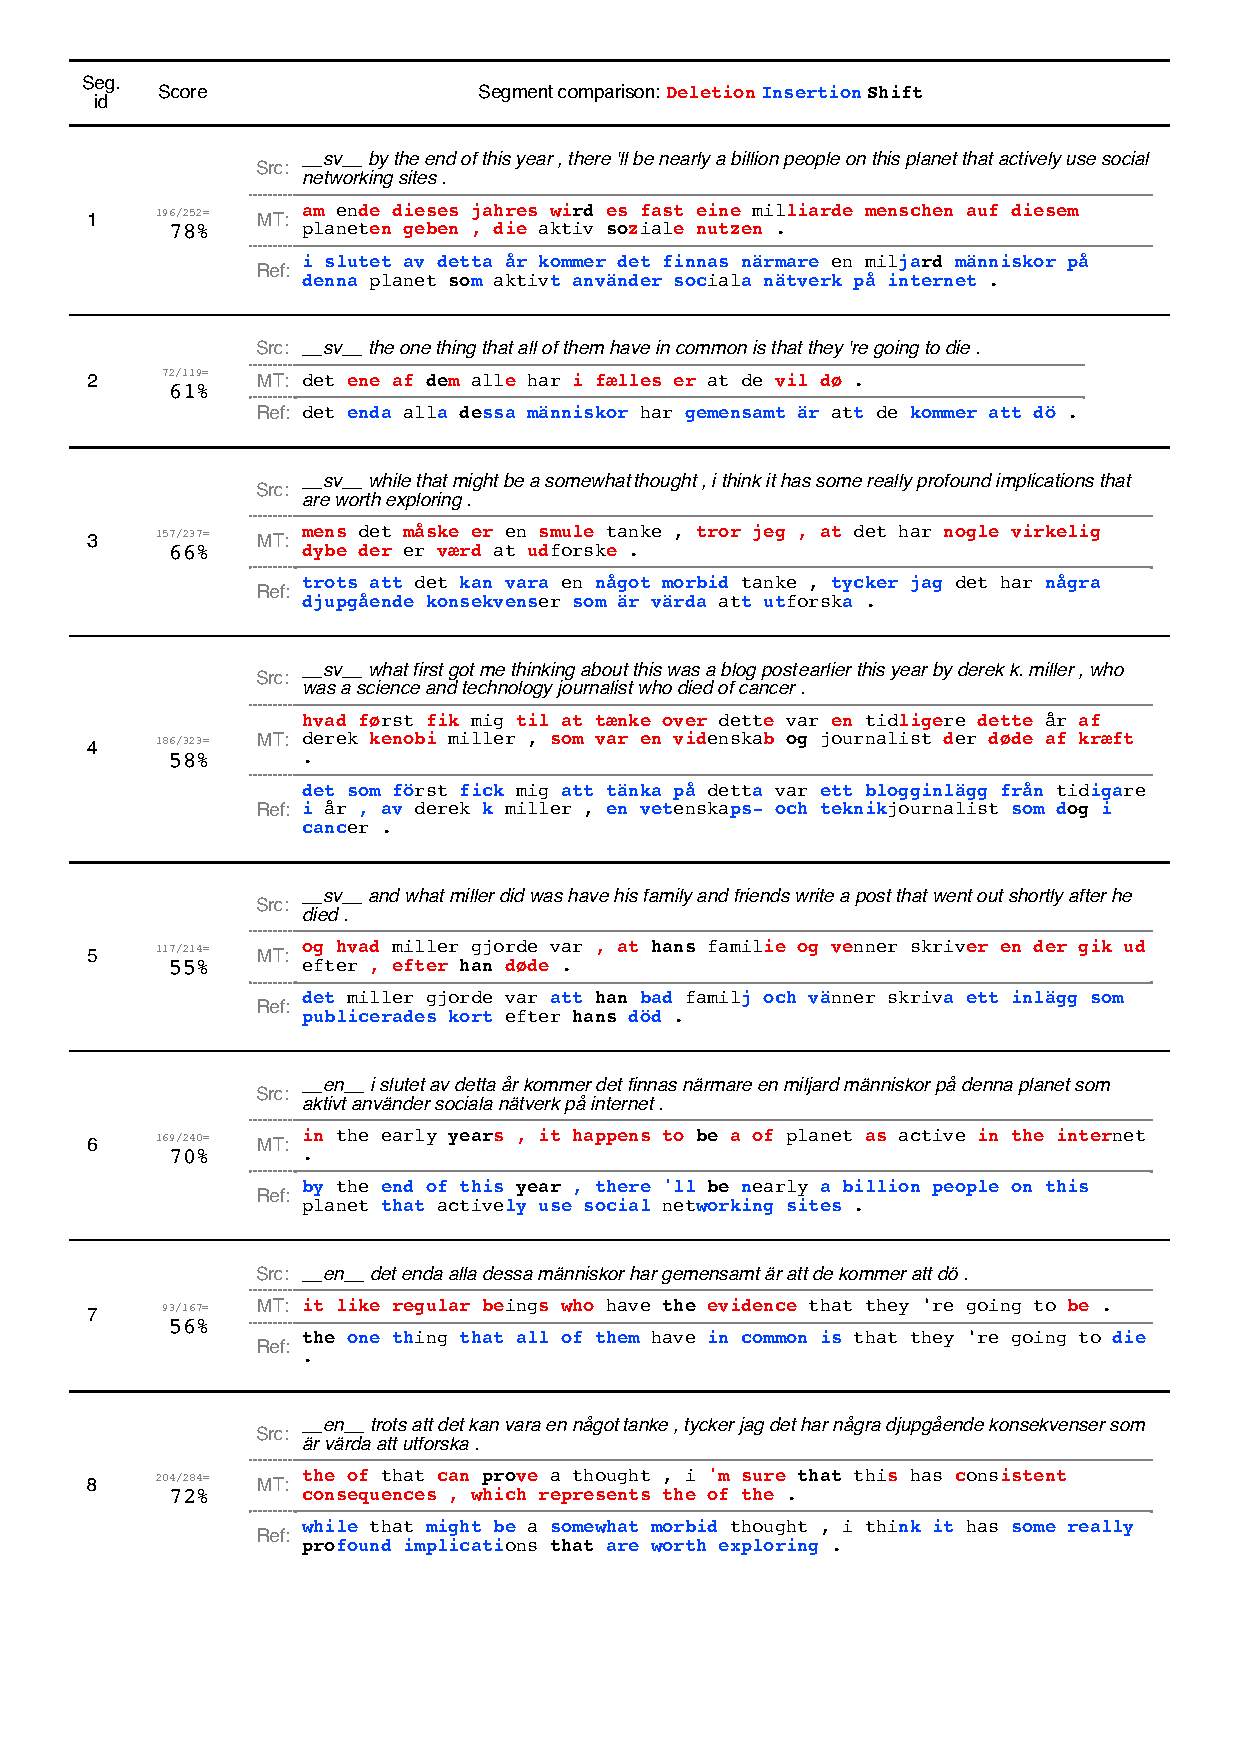
\includepdf[pages=-,scale=0.9,pagecommand={}]{mt_example_output/en+de+da+sv.pdf}

\printbibliography
\end{document}
